\documentclass[11pt,a4paper]{article}
\usepackage[margin=2.3cm]{geometry}
\usepackage[T1]{fontenc}
\usepackage{lmodern}
\usepackage{microtype}
\usepackage{amsmath,amssymb}
\usepackage{graphicx}
\usepackage{booktabs}
\usepackage{tabularx}
\usepackage{caption}
\usepackage{float}
\usepackage{xcolor}
\usepackage{enumitem}
\usepackage[numbers,sort&compress]{natbib}
\usepackage[colorlinks=true,linkcolor=blue!50!black,citecolor=blue!50!black,urlcolor=blue!50!black]{hyperref}
\captionsetup{font=small,labelfont=bf}
\setlist{itemsep=2pt,topsep=4pt}
\graphicspath{{figures/}}
\newcommand{\ci}[2]{\,[#1,\,#2]}

\title{\textbf{Predicting New User Engagement on Zindi}\\[4pt]
\large Do time-series foundation models help? A pre-registered study}
\author{Majid Alansari \and Ghaleb AlDoboni \and Ahmed AlMessabi\\[4pt]
\small AI7101 Machine Learning with Python \quad\textperiodcentered\quad Mohamed bin Zayed University of Artificial Intelligence}
\date{October 2026}

\begin{document}
\maketitle

\begin{abstract}
Online platforms depend not only on acquiring new users but also on retaining them. We study the Zindi
New User Engagement Prediction Challenge: predicting whether a newly registered user will be active in the
month after signup. The data are masked platform logs (12{,}413 users, about 317{,}000 activity events),
and only 11--20\% of new users return, so the problem is strongly imbalanced. We had two objectives: to
build a reliable engagement predictor from engineered behavioural features, and to test whether embeddings
from a modern time-series foundation model, TimesFM-3, add predictive information. Substantial data
preparation was required: we inferred the order of masked months, corrected a clock offset between tables,
prevented target leakage and removed an automatically generated badge event that distorted the label. Models
were evaluated with rolling-origin chronological splits, using F1, ROC-AUC and PR-AUC with paired-bootstrap
confidence intervals. The pre-registered TimesFM hybrid reached F1~$=0.459$ against $0.446$ for a tuned
LightGBM, but the improvement was statistically inconclusive; an ablation over the PCA dimension of the
embedding (2 to 128 components and the full 5{,}120-dimensional embedding) shows no setting that reliably improves ranking quality over
the baseline. In later exploratory work, CatBoost on engineered features reached F1~$=0.482$,
ROC-AUC~$=0.812$ and PR-AUC~$=0.505$, with confidence intervals above the baseline. A plausible explanation for
the limited value of TimesFM, supported by a diagnostic test but not established as the cause, is that its
per-series normalisation removes absolute activity level, one of the strongest predictors. The
best model is most useful as a ranking tool: the top 10\% of ranked users return at 3.9 times the base rate.
\end{abstract}

\section{Introduction}
User retention is a central challenge for online platforms: acquiring a user has limited value if they sign
up once and never return. Zindi, an African data-science competition platform, released masked logs of its
own users for the New User Engagement Prediction Challenge~\citep{zindi2022}. The task is binary
classification:
\[
y = \begin{cases} 1 & \text{if the user is active in the month after their signup month,}\\ 0 & \text{otherwise.}\end{cases}
\]
A reliable engagement score helps the platform rank new users for onboarding support, learning and
competition recommendations, or retention analysis, so that limited outreach effort goes where it matters.

Beyond the prediction task we asked a research question: \emph{do embeddings from a time-series foundation
model add predictive signal beyond well-designed handcrafted behavioural features?} A user's signup month is
a short time series of browsing, learning, competition and account activity; a pretrained model such as
TimesFM~\citep{das2024timesfm,timesfm3} might discover useful temporal patterns automatically. We fixed three
hypotheses and the decision rule for H3 \emph{before} running any foundation-model experiment
(pre-registration):
\begin{itemize}
  \item \textbf{H1:} TimesFM embeddings alone underperform a tuned gradient-boosting model on handcrafted features.
  \item \textbf{H2:} Smoothing sparse events into dense activity curves improves the TimesFM embeddings.
  \item \textbf{H3:} Handcrafted features plus TimesFM embeddings outperform the tuned tabular baseline.
\end{itemize}
The results were \emph{mixed} for H1, \emph{reversed} for H2 and \emph{inconclusive} for H3.

\section{Dataset and Problem Formulation}
\subsection{Data sources}
The challenge provides event logs rather than a model-ready table (Table~\ref{tab:sources}); we aggregated
many rows per user into one user-level record. All tables were loaded with \texttt{pandas}.

\begin{table}[H]
\centering\small
\begin{tabularx}{0.9\linewidth}{lrX}
\toprule
Table & Rows & Role in the project\\
\midrule
\texttt{UserActivity.csv} & 317{,}292 & Page views and platform actions\\
\texttt{Users.csv} & 12{,}413 & Signup time, country, masked user attributes\\
\texttt{CompetitionPartipation.csv} & 8{,}385 & Competition membership and submissions\\
\texttt{Discussion.csv} / \texttt{Comments.csv} & 1{,}439 / 467 & Community activity\\
Competition / Blog / Job metadata & 247 / 117 / 34 & Context for engineered features\\
\bottomrule
\end{tabularx}
\caption{Raw data sources. IDs and months are masked; the logs cover seven months.}
\label{tab:sources}
\end{table}

After aggregation the supervised-learning representation is $X \in \mathbb{R}^{9026\times 68}$ and
$y\in\{0,1\}^{9026}$: 9{,}026 labelled users from five signup cohorts (cohorts 0--4). Cohort 5 is Zindi's
hidden test set (labels unavailable) and cohort 6 has no following month. Only signup-month information enters
$X$; the following month is used only to compute $y$.

\subsection{Target construction}
The official definition counts any activity row in the following month. Our audit found a one-day
\texttt{badge\_OCZE} award recorded for 2{,}892 users: 99\% of these rows fall inside a two-hour window and
94\% of recipients did nothing else that day. Counting this passive award as engagement raised one cohort's
apparent active rate from 27\% to 77\% (Figure~\ref{fig:eda1}, left). Our primary target is therefore
\begin{quote}
\texttt{label\_engaged} = at least one activity in the month after signup, excluding \texttt{badge\_*} events
and confirmed system-wide batch events.
\end{quote}
Because this differs from the official label, we also report the official ``any activity'' label as a
sensitivity analysis (Section~\ref{sec:sensitivity}).

\section{Data Preparation}
Data preparation was one of the most important stages; Table~\ref{tab:prep} summarises each step and its
motivation.

\begin{table}[H]
\centering\small
\begin{tabularx}{\linewidth}{>{\raggedright\arraybackslash}p{2.7cm}XX}
\toprule
Step & What we did & Why\\
\midrule
Month order & Ordered the masked codes $11\to12\to1\to\dots\to5$ & Of all 5{,}040 orders, only this one leaves almost no events before signup (0.071\% vs 0.187\% for the next best)\\
Clock alignment & Shifted \texttt{UserActivity} by $-2$\,h, then $-1$\,h after a detected switch & Its clock ran ahead of the other tables; afterwards 99.94\% of ``Signed Up'' events coincide with signup\\
Target & Excluded badge and batch events from the label & A one-day badge batch inflated one cohort from 27\% to 77\%\\
Leakage guard & Features from the signup month $t$ only; $y$ from month $t{+}1$ & The model sees only what is known at prediction time; enforced by unit tests\\
Missing values & Missing country $\to$ its own category; absent behaviour $\to$ zero counts & 28\% of users lack a country; missingness is informative\\
Categoricals & Country and two attributes as native categories, levels fitted on training data & 123 countries make one-hot encoding sparse; avoids leaking unseen levels\\
Duplicates & Dropped ``Joined Competition'' activity rows & 98.75\% duplicate a participation-table record\\
Scaling & $\log(1+x)$ and standardisation for linear models only & Counts are heavy-tailed; trees do not need it\\
\bottomrule
\end{tabularx}
\caption{Data preparation steps and their motivation.}
\label{tab:prep}
\end{table}

\paragraph{Feature engineering.} Features answer three questions: \emph{how much} the user did,
\emph{how recently and regularly}, and \emph{in what context}. For each behaviour group (browse, learn,
compete, contribute, account, onboarding, badges, comments) we compute the event count, active days, recency
to month end, activity span, last-7-day count and rate. We add session statistics, the position of the last
active day within the observed window, activity trend, the number of days observed (late signups have
shorter windows), and \emph{competition liveness}: how many distinct users were active in the user's
competitions during the last week of the month.

\section{Exploratory Data Analysis}
Figures~\ref{fig:eda1}--\ref{fig:eda3} were produced with Seaborn in the accompanying notebook.

\begin{figure}[H]
\centering
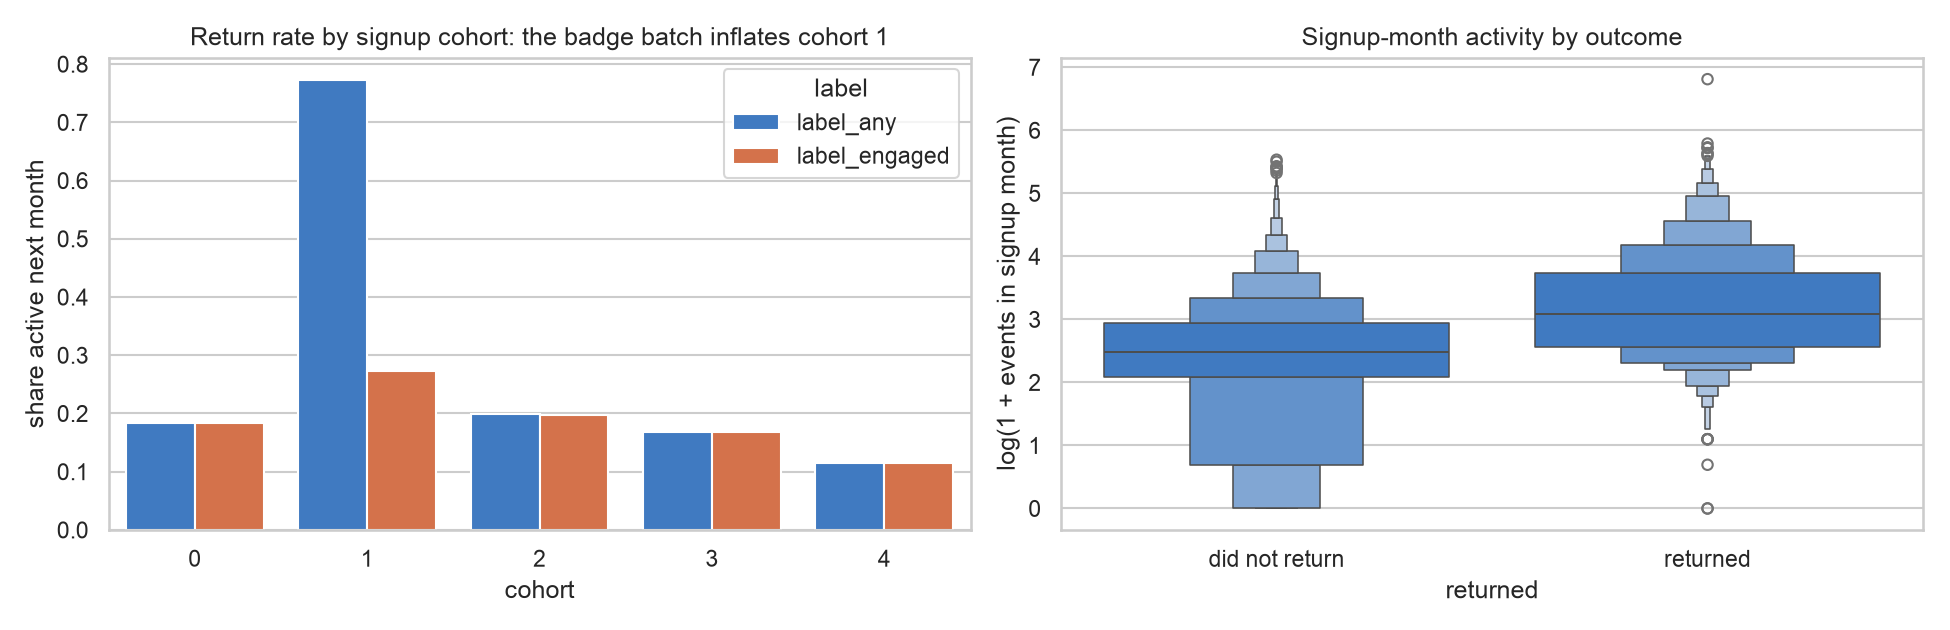
\includegraphics[width=\linewidth]{eda_cohorts_activity.png}
\caption{\textbf{Left:} next-month return rate by signup cohort under the official label (\texttt{label\_any})
and our cleaned label; the badge batch inflates cohort 1. \textbf{Right:} signup-month activity
($\log(1+\text{events})$) by outcome. Returners are more active, but the distributions overlap heavily.}
\label{fig:eda1}
\end{figure}

\paragraph{Class imbalance and temporal drift.} The return rate falls across later cohorts
($19.8\%\to16.9\%\to11.5\%$). This has two consequences: accuracy is misleading (an all-negative classifier
scores 88.5\% on cohort 4 with F1~$=0$), and random cross-validation would mix cohorts and overstate quality.

\begin{figure}[H]
\centering
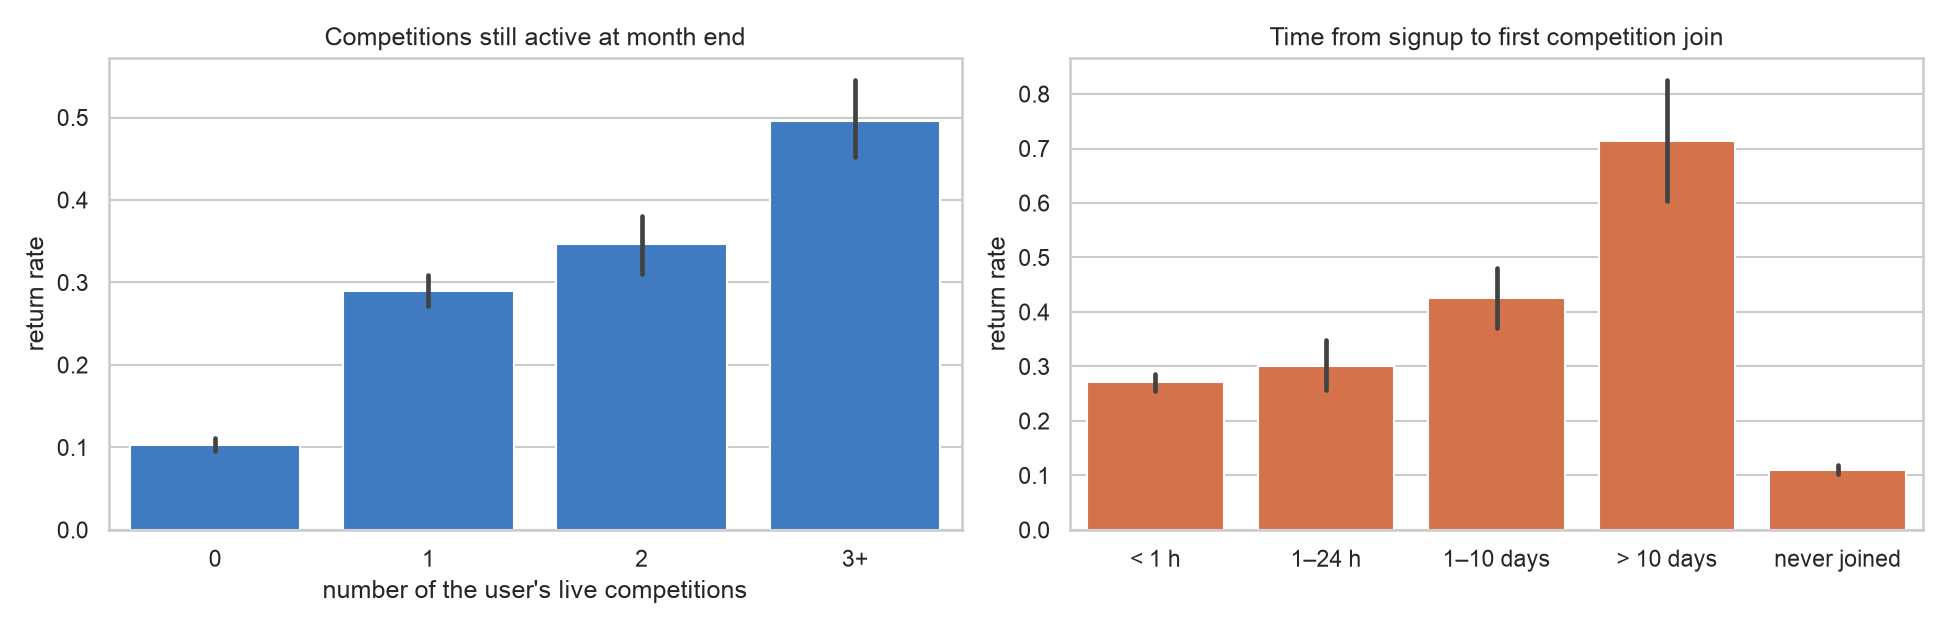
\includegraphics[width=\linewidth]{eda_competitions.png}
\caption{Return rate by the number of the user's competitions still active at month end (left) and by time
from signup to the first competition join (right), all labelled cohorts, 95\% confidence intervals.}
\label{fig:eda2}
\end{figure}

\paragraph{Competition context.} Competition liveness is the clearest pattern. On the training cohorts 0--2,
users with 0, 1, 2 and 3+ live competitions return at 13\%, 35\%, 43\% and 65\%. Join timing also matters:
users who first join within one hour return at 32\%, within a day 46\%, after 1--10 days 60\% and after more
than 10 days 76\%, against 14\% for users who never join. A later join signals continuing interest, while
an immediate join is often a one-off visit through a competition link. Users whose first real action was a
competition page return at only about 4\%, against 26--28\% for those who start by browsing or learning.
These are associations, not causal effects; they motivated the liveness and recency features.

\begin{figure}[H]
\centering
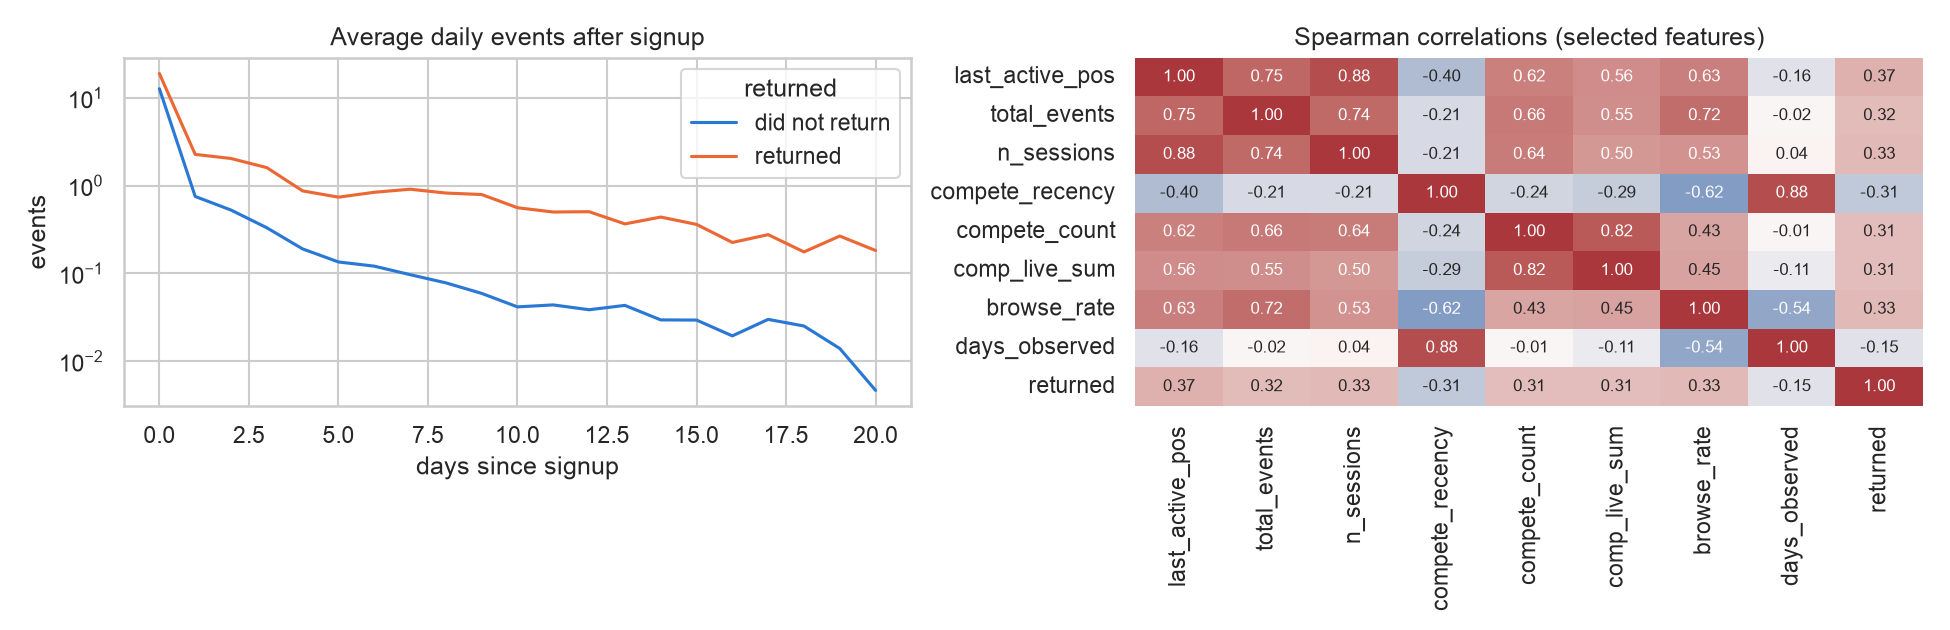
\includegraphics[width=\linewidth]{eda_daily_corr.png}
\caption{\textbf{Left:} average daily events after signup (log scale): returners keep coming back on later
days. \textbf{Right:} Spearman correlations between selected features and the outcome.}
\label{fig:eda3}
\end{figure}

\paragraph{Recency over volume.} Almost every user is active on signup day; returners differ in coming back
on later days, so recency and the last-active position matter more than raw volume. Many activity features
are strongly correlated, which favours tree ensembles. Finally, 9.1\% of users have no signup-month events and
return at only 0.24\%; 778 of them never appear in any table and are probably untracked.

\section{Evaluation Methodology}
\subsection{Rolling-origin chronological validation}
Because return rates drift, we validate the way the model would be used: train on past cohorts, tune on the
next and test on the one after (Table~\ref{tab:folds}). The validation cohort is used for hyperparameter
search, early stopping and the decision threshold; the test cohorts are never used for any choice. Every
fitted object (scalers, PCA, category levels) sees training data only.

\begin{table}[H]
\centering\small
\begin{tabular}{lccc}
\toprule
Fold & Training cohorts & Validation cohort & Test cohort\\
\midrule
A & 0--1 & 2 & 3\\
B & 0--2 & 3 & 4\\
\bottomrule
\end{tabular}
\caption{Rolling-origin folds (4{,}278 test users in total). Zindi's hidden cohort is not used: its labels are unavailable.}
\label{tab:folds}
\end{table}

\subsection{Metrics and statistical testing}
F1 is the primary metric (the competition metric):
\[
\text{Precision}=\frac{TP}{TP+FP},\qquad \text{Recall}=\frac{TP}{TP+FN},\qquad
F_1=\frac{2\,\text{Precision}\cdot\text{Recall}}{\text{Precision}+\text{Recall}},
\]
with the threshold tuned on validation. We also report ROC-AUC and PR-AUC, which are threshold-free and
robust to the drifting base rate; PR-AUC focuses on ranking the rare positive class. Tree models are averaged
over five random seeds. Model differences are tested with a paired bootstrap~\citep{efron1993bootstrap}
(2{,}000 resamples, the same resampled users for both models within each fold), giving 95\% confidence
intervals for F1, ROC-AUC and PR-AUC.

\subsection{Pre-registration and test isolation}
For the TimesFM experiment, the hypothesis, the candidate-selection rule (highest mean \emph{validation}
PR-AUC) and the verdict rule were written down before any TimesFM model was evaluated: \emph{supported} if the
pooled confidence intervals for F1 and PR-AUC are both above zero, \emph{partial} if only an AUC interval is,
\emph{inconclusive} if all intervals include zero, and \emph{not supported} if all point estimates are
$\le 0$. Later exploratory models were developed on validation only, and their final list was fixed before a
single test evaluation.

\section{Models and Hyperparameters}
\begin{itemize}
  \item \textbf{Logistic regression} (B1): interpretable linear reference; class-balanced, on $\log(1+x)$-scaled features.
  \item \textbf{LightGBM}~\citep{ke2017lightgbm} (B3): the main strong tabular baseline.
  \item \textbf{MiniRocket}~\citep{dempster2021minirocket} (B4): random convolutional features of the raw daily series, followed by logistic regression.
  \item \textbf{TimesFM-3 models} (P1--P4): embeddings of each user's activity series, alone or as PCA components inside LightGBM.
  \item \textbf{CatBoost}~\citep{prokhorenkova2018catboost} (N2): final exploratory model with native categorical handling.
\end{itemize}

\begin{table}[H]
\centering\small
\begin{tabularx}{\linewidth}{lXX}
\toprule
Model & Search (validation only) & Selected setting\\
\midrule
LightGBM & 30-trial random search per fold over leaves $\{3,4,7,15,31,63\}$, min.\ child samples $\{10,20,50,100\}$, learning rate $\{.01,.03,.05\}$, subsample $\{.7,.8,1\}$, column sample $\{.5,.8,1\}$, L2 $\{0,1,5\}$; early stopping on validation & Fold A: 15 leaves, lr 0.03, L2 0; Fold B: 4 leaves, lr 0.05, L2 5 (both: min.\ child 50, subsample 0.7, colsample 0.5). Frozen and reused for all hybrids\\
CatBoost & 14-configuration random search over depth 3--8, L2 1--20, learning rate 0.02--0.05, random strength, bagging temperature & Depth 4, lr 0.03, L2 5 (search best 0.560 vs 0.559 val.\ PR-AUC: a plateau)\\
Logistic regression & $C$ chosen on validation PR-AUC for embedding models & Balanced class weights\\
MiniRocket + LR & $C\in\{10^{-6},\dots,10^{-1}\}$ on validation PR-AUC & $C=10^{-5}$ / $10^{-4}$\\
Threshold & F1-maximising threshold on validation, grid 0.02--0.98 & Applied unchanged to test\\
\bottomrule
\end{tabularx}
\caption{Hyperparameter search. Shallow trees won consistently: the signal consists of a few strong effects rather than deep interactions.}
\label{tab:hparams}
\end{table}

\section{TimesFM-3 Foundation-Model Experiments}
\subsection{Embedding extraction}
Each user's signup month was represented as four daily activity series (browse, learn, compete, account),
either raw (31 daily counts) or kernel-smoothed into a dense intensity curve (512 points). Each series was
passed through TimesFM-3 (330M parameters, 20 transformer layers, width 1{,}280) and the hidden states of the
last layer were mean-pooled, giving $4\times1{,}280=5{,}120$ numbers per user. Hybrid models compress this
embedding with PCA (fitted on training data) and append the components to the handcrafted features.

\subsection{Pre-registered result}
The validation-selected candidate was P4 with 8 PCA components of the smoothed-series embedding (mean
validation PR-AUC $=0.5394$).

\begin{table}[H]
\centering\small
\begin{tabular}{lccc}
\toprule
Model & F1 & ROC-AUC & PR-AUC\\
\midrule
Tuned LightGBM (B3) & 0.446 & 0.794 & 0.472\\
Selected TimesFM hybrid (P4, PCA 8) & 0.459 & 0.795 & 0.474\\
\midrule
Difference, 95\% CI & $+0.013\ci{-0.001}{+0.027}$ & $+0.001\ci{-0.002}{+0.004}$ & $+0.002\ci{-0.003}{+0.008}$\\
\bottomrule
\end{tabular}
\caption{Pre-registered comparison on the test cohorts. All intervals include zero: the verdict is \textbf{inconclusive}.}
\label{tab:prereg}
\end{table}
An inconclusive result does not prove that TimesFM has zero value. The 95\% intervals are compatible with no
improvement and with improvements of up to roughly 0.03 F1 and 0.01 PR-AUC; under the assumptions of the
bootstrap analysis (two test cohorts, resampling of users within each cohort), substantially larger gains are
unlikely, but this is a statement of uncertainty, not a guaranteed upper bound, and effects could differ on
other cohorts or platforms.

\subsection{Ablation: PCA dimension versus the full embedding}\label{sec:pca}
To test whether the inconclusive result depends on how strongly the embedding is compressed, we varied the
number of PCA components appended to the handcrafted features ($k\in\{2,4,8,16,32,64,128\}$) and also used the
full standardised 5{,}120-dimensional embedding without PCA, for both the raw-series and smoothed-series
embeddings. All other settings (frozen LightGBM hyperparameters, five seeds, folds) were unchanged, and
$k=0$ is the LightGBM baseline (Figure~\ref{fig:pca}, Table~\ref{tab:pca}).
\begin{figure}[H]\centering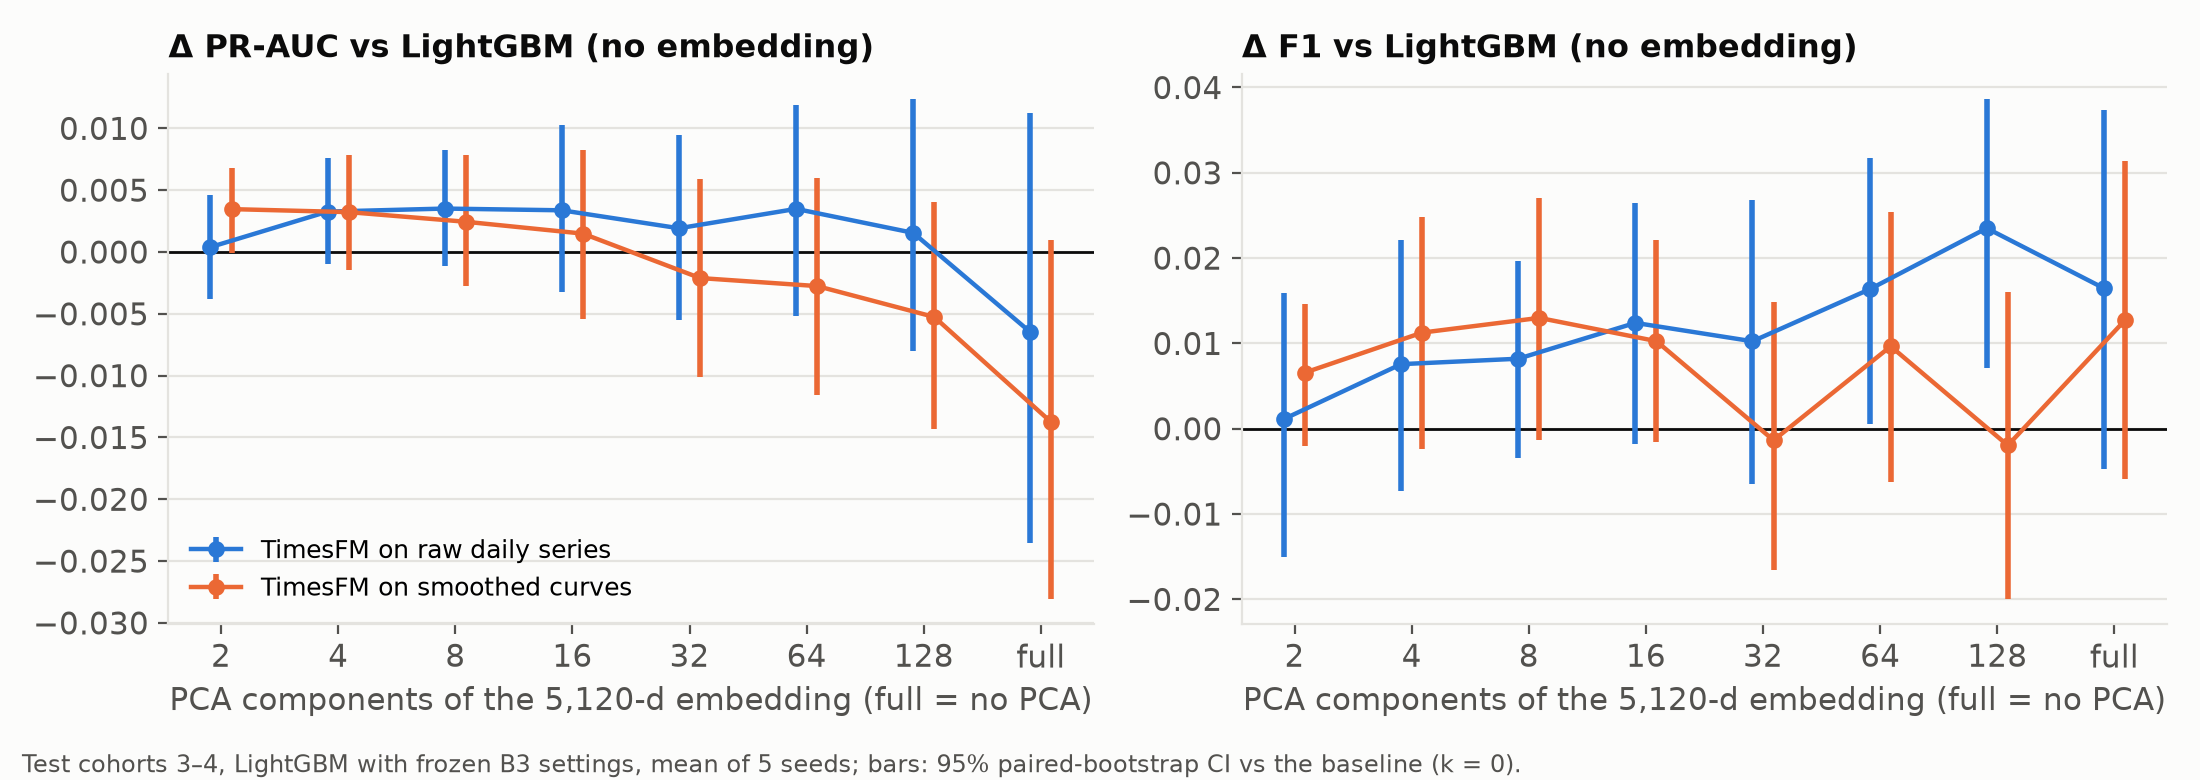
\includegraphics[width=\linewidth]{fig_pca_ablation.png}
\caption{Effect of the number of PCA components of the TimesFM-3 embedding on test PR-AUC and F1,
relative to the LightGBM baseline without embeddings. Bars are 95\% paired-bootstrap confidence intervals.}
\label{fig:pca}\end{figure}
\begin{table}[H]\centering\small\setlength{\tabcolsep}{4pt}
\begin{tabular}{llccccc}\toprule
Embedding & $k$ & Expl.\ var. & Val.\ PR-AUC & Test PR-AUC & $\Delta$PR-AUC [95\% CI] & $\Delta$F1 [95\% CI]\\\midrule
none (LightGBM) & 0 & -- & 0.537 & 0.472 & -- & --\\\midrule
raw daily series & 2 & 0.51 & 0.536 & 0.472 & $+0.000$\,[$-0.004$, $+0.005$] & $+0.001$\,[$-0.015$, $+0.016$]\\
raw daily series & 4 & 0.76 & 0.537 & 0.475 & $+0.003$\,[$-0.001$, $+0.008$] & $+0.008$\,[$-0.007$, $+0.022$]\\
raw daily series & 8 & 0.87 & 0.537 & 0.475 & $+0.004$\,[$-0.001$, $+0.008$] & $+0.008$\,[$-0.003$, $+0.020$]\\
raw daily series & 16 & 0.92 & 0.538 & 0.475 & $+0.003$\,[$-0.003$, $+0.010$] & $+0.012$\,[$-0.002$, $+0.026$]\\
raw daily series & 32 & 0.95 & 0.535 & 0.474 & $+0.002$\,[$-0.006$, $+0.009$] & $+0.010$\,[$-0.006$, $+0.027$]\\
raw daily series & 64 & 0.97 & 0.532 & 0.475 & $+0.003$\,[$-0.005$, $+0.012$] & $+0.016$\,[$+0.001$, $+0.032$]$^{*}$\\
raw daily series & 128 & 0.99 & 0.528 & 0.473 & $+0.002$\,[$-0.008$, $+0.012$] & $+0.024$\,[$+0.007$, $+0.039$]$^{*}$\\
raw daily series & full & 1.00 & 0.534 & 0.465 & $-0.006$\,[$-0.024$, $+0.011$] & $+0.016$\,[$-0.005$, $+0.037$]\\
\midrule
smoothed curves & 2 & 0.33 & 0.534 & 0.475 & $+0.003$\,[$-0.000$, $+0.007$] & $+0.007$\,[$-0.002$, $+0.015$]\\
smoothed curves & 4 & 0.46 & 0.538 & 0.475 & $+0.003$\,[$-0.001$, $+0.008$] & $+0.011$\,[$-0.002$, $+0.025$]\\
smoothed curves & 8 & 0.62 & 0.539 & 0.474 & $+0.002$\,[$-0.003$, $+0.008$] & $+0.013$\,[$-0.001$, $+0.027$]\\
smoothed curves & 16 & 0.78 & 0.540 & 0.473 & $+0.001$\,[$-0.005$, $+0.008$] & $+0.010$\,[$-0.002$, $+0.022$]\\
smoothed curves & 32 & 0.89 & 0.538 & 0.470 & $-0.002$\,[$-0.010$, $+0.006$] & $-0.001$\,[$-0.017$, $+0.015$]\\
smoothed curves & 64 & 0.95 & 0.538 & 0.469 & $-0.003$\,[$-0.012$, $+0.006$] & $+0.010$\,[$-0.006$, $+0.025$]\\
smoothed curves & 128 & 0.98 & 0.532 & 0.467 & $-0.005$\,[$-0.014$, $+0.004$] & $-0.002$\,[$-0.020$, $+0.016$]\\
smoothed curves & full & 1.00 & 0.529 & 0.458 & $-0.014$\,[$-0.028$, $+0.001$] & $+0.013$\,[$-0.006$, $+0.031$]\\
\bottomrule
\end{tabular}
\caption{PCA-dimension ablation (test cohorts 3--4). $^{*}$: confidence interval excludes zero.
Explained variance is the share of embedding variance kept by the PCA components (mean over folds).}
\label{tab:pca}\end{table}
No compression level turns the embedding into a reliable gain in ranking quality: every PR-AUC confidence interval includes zero and all differences are within $\pm0.004$, except that adding more components of the smoothed-curve embedding steadily \emph{hurts} (down to $-0.014$ with the full embedding), consistent with extra dimensions adding noise. For the raw-series embedding, F1 drifts upward with $k$ (from $+0.001$ at $k=2$ to $+0.024$ at $k=128$), and two settings ($k=64$, $k=128$) have F1 intervals just above zero. We read this cautiously: the trend does not appear in the threshold-free PR-AUC, validation PR-AUC \emph{decreases} with $k$ (so these settings would not have been selected), and with 16 settings tested about one such interval is expected by chance. Overall, the ablation is consistent with the explanation offered in Section~\ref{sec:why}: if normalisation has removed the activity level, neither compressing nor expanding the embedding can restore it.


\section{Why the Foundation Model May Not Have Helped}\label{sec:why}
TimesFM normalises each input series by its own level and spread (reversible instance
normalisation~\citep{kim2022revin}). In our smoke test a series and the same series multiplied by 100 produced
identical embeddings, $\cos\big(e(x), e(100x)\big)=1.000$. For engagement this is likely to be harmful: a
user with 1 event on day 5 and a user with 100 events on day 5 become indistinguishable, although activity
level is highly predictive. We offer this as a plausible explanation rather than an established cause; other
factors may contribute, such as the shortness and sparsity of 31-day series, which differ from the long, dense
series TimesFM was pretrained on. Three further diagnostics are consistent with it, without proving it. A
scale-aware variant (a fixed reference patch prepended to every series) made the embeddings level-sensitive
but did not improve validation performance, possibly because magnitude is already captured by the count
features. Zero-shot TimesFM forecasts of next-month activity were weaker than a simple event count. A custom
multi-view network that learns per-user weights over its inputs put only 4--5\% of its weight on the
TimesFM view.

\begin{figure}[H]
\centering
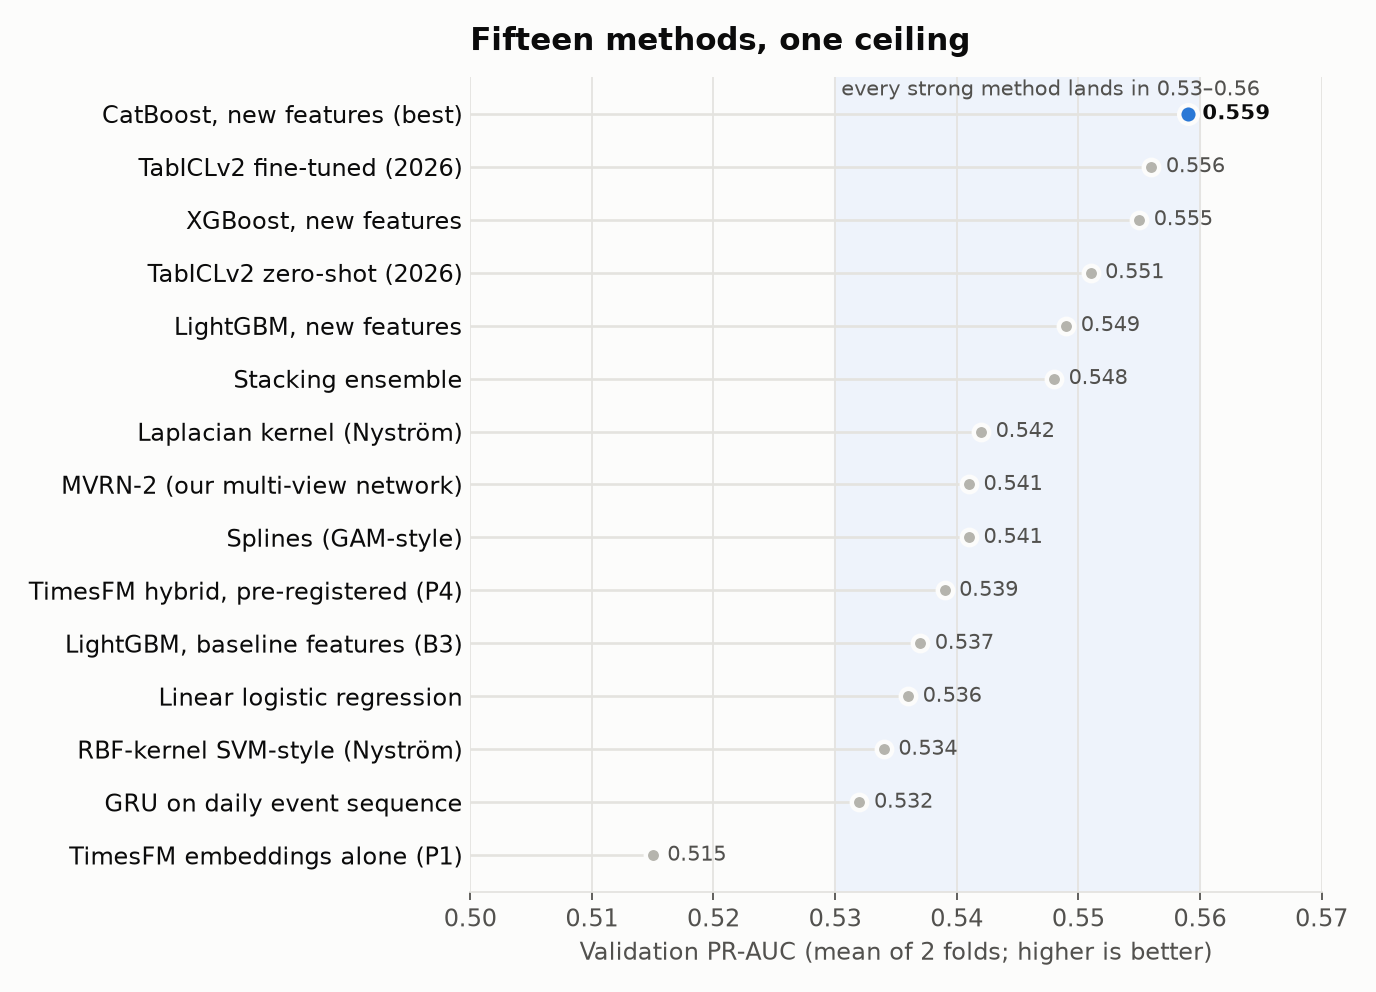
\includegraphics[width=0.8\linewidth]{methods_ceiling.png}
\caption{Validation PR-AUC of fifteen methods, including linear and kernel models, XGBoost, stacking, a GRU,
the tabular foundation model TabICLv2~\citep{qu2025tabicl,tabiclv2} and custom networks. All lie between
0.53 and 0.56, suggesting that the information in a user's first month, not model capacity, is the limit.}
\label{fig:ceiling}
\end{figure}

\section{Final CatBoost Model and Results}
The preferred model, N2, is CatBoost on the handcrafted, session/trend and competition-liveness features,
refit on training plus validation data after selection.

\begin{table}[H]
\centering\small
\begin{tabular}{lccc}
\toprule
Model (test cohorts 3--4, mean) & F1 & ROC-AUC & PR-AUC\\
\midrule
Rule: active in last 7 days (B0) & 0.395 & 0.691 & 0.233\\
Logistic regression (B1) & 0.453 & 0.778 & 0.456\\
Tuned LightGBM (B3) & 0.446 & 0.794 & 0.472\\
MiniRocket (B4) & 0.457 & 0.788 & 0.467\\
TimesFM hybrid, pre-registered (P4) & 0.459 & 0.795 & 0.474\\
\textbf{CatBoost + engineered features (N2)} & \textbf{0.482} & \textbf{0.812} & \textbf{0.505}\\
Ensemble including TimesFM (N4) & 0.496 & 0.813 & 0.501\\
\bottomrule
\end{tabular}
\caption{Test results.}
\label{tab:results}
\end{table}

\begin{figure}[H]
\centering
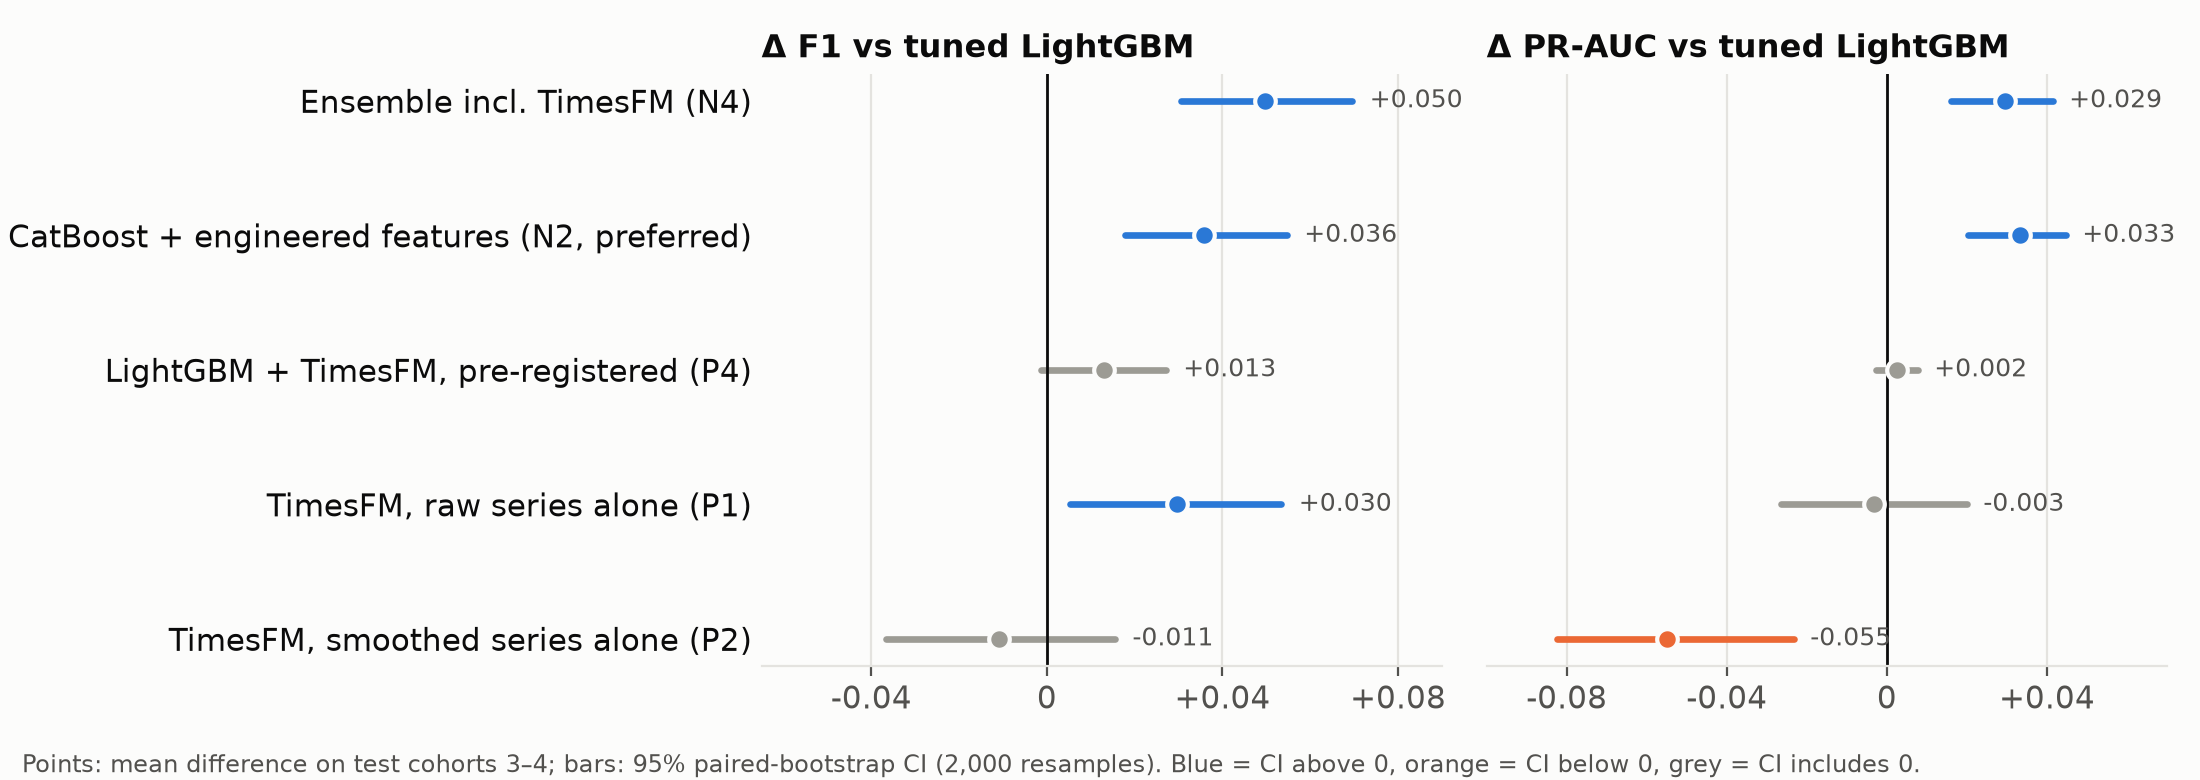
\includegraphics[width=\linewidth]{fig_ci_forest.png}
\caption{Differences from tuned LightGBM with 95\% paired-bootstrap confidence intervals. N2 improves F1 by
$+0.036\ci{+0.018}{+0.055}$ and PR-AUC by $+0.033\ci{+0.020}{+0.045}$. N4 has the highest F1, but its
difference from N2 is not significant (F1 $+0.014\ci{-0.004}{+0.032}$), so the simpler N2 is preferred.}
\label{fig:forest}
\end{figure}

\begin{figure}[H]
\centering
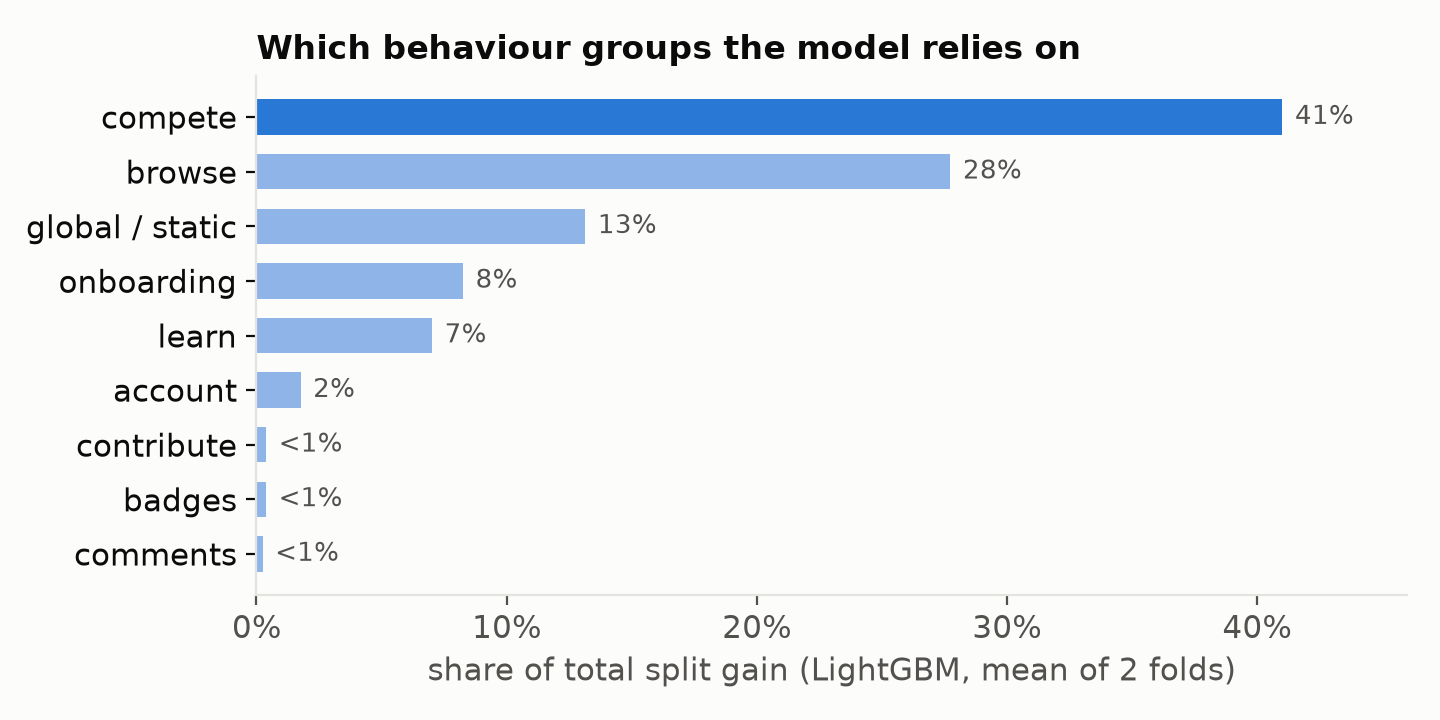
\includegraphics[width=0.66\linewidth]{fig_feature_groups.png}
\caption{Share of LightGBM split gain by behaviour group: competition and browsing behaviour dominate;
badges, comments and contributions add almost nothing. Removing the competition features costs
$-0.046$ F1 in an ablation.}
\label{fig:importance}
\end{figure}

\section{Error Analysis}
Users with more than 20 signup-month events are ranked well (within-segment AUC about 0.80). Users with 6--20
events make up 48\% of returners but are hard to separate (AUC about 0.69), as are users without competition
activity (24\% of returners, AUC about 0.67). Users with no signup-month events (9.1\%) return at 0.24\%;
embeddings cannot help this group by construction.

\section{Sensitivity Analysis}\label{sec:sensitivity}
\paragraph{Never-tracked users.} Removing the 778 probably untracked users leaves F1 and PR-AUC unchanged for
all models; ROC-AUC drops by about 0.015--0.02 for every model alike. The TimesFM verdict stays inconclusive.

\paragraph{Official Zindi label.} Training on the official ``any activity'' label reduces F1 to 0.386 for
LightGBM and 0.384 for the TimesFM hybrid (from 0.446 and 0.459), and makes the hybrid significantly worse
than LightGBM on ROC-AUC and PR-AUC. Constructing the target carefully matters.

\paragraph{Leaderboard context.} The competition's top private scores (0.85--0.87) are not comparable F1
values: a confirmed duplicate-ID scoring bug inflated F1, and the re-scored top entries match the accuracy of
predicting that nobody returns (0.853). Legitimate entries cluster at 0.42--0.51 F1.

\section{Practical Applicability}
The model is most useful as a ranking system (Table~\ref{tab:lift}).
\begin{table}[H]
\centering\small
\begin{tabular}{lccc}
\toprule
Users contacted (ranked by N2) & Precision & Lift over base rate & Share of all returners reached\\
\midrule
Top 5\% & 0.664 & 4.7$\times$ & 23\%\\
Top 10\% & 0.556 & 3.9$\times$ & 39\%\\
Top 20\% & 0.424 & 3.0$\times$ & 60\%\\
\bottomrule
\end{tabular}
\caption{Ranking quality on the test cohorts (base rate 0.142).}
\label{tab:lift}
\end{table}
Applications include prioritising onboarding help, recommending competitions and learning content, and
allocating limited community-outreach effort. The model predicts \emph{who} is likely to return, not who would
return \emph{because} Zindi contacts them; estimating business impact requires a controlled experiment that
compares model-guided outreach, random outreach and a no-outreach control.

\section{Related Work}
New-user churn has been studied on question-answering sites~\citep{dror2012churn}, mobile social
apps~\citep{yang2018clus}, MOOCs~\citep{feng2019dropout} and subscription services~\citep{gregory2018churn}. The
recurring recipe is engineered temporal and context features with gradient boosting; recent event-sequence
benchmarks report recurrent models best on short sequences and aggregated features within about 5\% of
them~\citep{osin2025ebes}. Applying these approaches to our data (time-window and recency features, context
normalisation, stacking, a GRU and TabICLv2) gave no gain over N2, consistent with Figure~\ref{fig:ceiling}.

\section{Limitations}
\begin{itemize}
  \item The data are masked, so the month order and calendar were inferred rather than confirmed by Zindi.
  \item Only five labelled cohorts and two primary test folds are available.
  \item The primary target excludes a passive badge batch and therefore differs from the official label.
  \item First-month behaviour is short and sparse; many returners resemble users who never return.
  \item Some users appear untracked rather than inactive.
  \item The base rate drifts, so a fixed threshold may not stay optimal.
  \item The CatBoost result is exploratory and combines three changes (features, model, refit), whose individual contributions are not isolated.
\end{itemize}

\section{Discussion and Conclusion}
Better understanding of the data produced more value than model complexity. A plausible reason TimesFM added
little is that its normalisation removes absolute activity level, which appears to matter most for retention;
the engineered features (returning across days, participating in live competitions, joining later rather than
immediately, being active near the month end) supplied the context the foundation model lacks. Chronological validation produced lower but realistic
estimates, and the highest test number was not automatically chosen: N4's F1 gain over N2 was not
significant.

The preferred CatBoost model reached F1~$=0.482$, ROC-AUC~$=0.812$ and PR-AUC~$=0.505$, a statistically
supported improvement over tuned LightGBM, while the pre-registered TimesFM hypothesis was not established.
Useful prediction is possible, but the strongest gains came from data quality, leakage-safe evaluation and
engineered features, not from the foundation model.

\paragraph{Future work.} Evaluate on further cohorts; study the difficult 6--20-event segment; test sequence
models that preserve absolute scale; and run a randomised outreach experiment to move from return prediction
to uplift modelling.

\paragraph{Reproducibility.} Code, the executed notebook and all result files:
\url{https://github.com/GhalebAldoboni/zindi-engagement-timesfm}. The Zindi data are not redistributed.

\bibliographystyle{plainnat}
\bibliography{references}
\end{document}
